% main.tex -- "Paraphrase-Resistant Detection of AI-Driven Code Rewrites:
% A Falsifiable Harness Applied to the chardet v6 to v7 Relicensing
% Dispute".
%
% Builds with stock TeX Live (pdflatex + bibtex). Packages used are all
% standard; nothing requires CTAN downloads on a default install.

\documentclass[11pt,letterpaper]{article}

\usepackage[T1]{fontenc}
\usepackage[utf8]{inputenc}
\usepackage{lmodern}
\usepackage{microtype}
\usepackage[margin=1in]{geometry}
\usepackage{graphicx}
\usepackage{booktabs}
\usepackage{tabularx}
\usepackage{xcolor}
\usepackage{listings}
\usepackage{enumitem}
\usepackage[hyphens]{url}
\usepackage[hidelinks]{hyperref}
\usepackage[capitalise,noabbrev]{cleveref}
\usepackage{titlesec}

% Spacing -- slightly tighter than article default but still arXiv-conventional.
\setlength{\parskip}{4pt}
\setlength{\parindent}{0pt}
\setlength{\emergencystretch}{3em}
\titlespacing*{\section}{0pt}{1.5ex plus .2ex}{0.8ex plus .2ex}
\titlespacing*{\subsection}{0pt}{1.2ex plus .2ex}{0.5ex plus .2ex}

% Listings style for the small code excerpts.
\definecolor{codebg}{gray}{0.96}
\lstset{
  basicstyle=\ttfamily\small,
  backgroundcolor=\color{codebg},
  frame=single,
  framerule=0pt,
  xleftmargin=1em,
  framexleftmargin=1em,
  breaklines=true,
  showstringspaces=false,
  columns=fullflexible,
  keepspaces=true,
  captionpos=b,
}
\lstdefinelanguage{toml}{
  morekeywords={true,false},
  morestring=[b]",
  morecomment=[l]\#,
  sensitive=true,
}

% Title block.
\title{\bfseries Paraphrase-Resistant Detection of AI-Driven Code Rewrites:\\
A Falsifiable Harness Applied to the chardet v6 to v7 Relicensing Dispute}

\author{
  Werner Kasselman \\
  Verivus OSS \\
  \texttt{werner@verivus.com}
}

\date{}

\begin{document}
\maketitle

\begin{abstract}
In March 2026 the maintainer of the Python \texttt{chardet} library
released version 7.0.0 as an MIT-licensed ``ground-up rewrite,''
produced with an LLM-driven coding agent, of a codebase that had
carried an LGPL licence since 2008. The relicensing drew objection
immediately, with critics arguing that any rewrite informed by an
LLM that had seen the original cannot be a clean-room
reimplementation and therefore cannot strip the original's
copyleft (an argument that is going to come up again, repeatedly,
as more production codebases get the same treatment). I am not
trying to adjudicate the chardet dispute, and this paper does not
take a position on whether v7's relicensing is valid; what I am
trying to do is move the conversation from assertion to evidence,
by shipping a detection harness that produces six structural,
falsifiable, reproducible signals comparing v6.0.0 and v7.0.0 of
the library, five of which are explicitly designed to survive
identifier renaming and module restructuring, and one of which
(AUX1, the file-hash baseline) is retained as a continuity check
with naive prior approaches. On the actual artefacts, literal
source carryover is zero, v7's call-graph topology is 0.881
similar to v6's, the normalised AST control-flow histogram cosine
is 0.984, three of five shared public-API signatures are
byte-identical (``strict''), v7 imports a substantially different
third-party dependency set (Jaccard 0.333), and the two versions
never agree on encoding or confidence over 1000 random byte
inputs. The combined picture is internally consistent but legally
ambiguous, with the honest summary being that v7 preserves the
\emph{shape of v6's thinking} while replacing what v6 actually
\emph{does}. The contribution is the methodology and the bundle,
not a verdict on chardet specifically (a self-contained,
multi-LLM-reviewed artefact that any reviewer, lawyer, or court
can re-run and inspect), sitting in a lineage of prior Verivus
work on Verifiable AI Governance (the ``AI You Can Prove'' thesis,
of which the DAG-TOML specification this proof bundle conforms to
is the current open-source instantiation, and of which sqry, the
AST-graph code-search tool used to corroborate the call-graph
findings, is a sibling instantiation).
\end{abstract}

\section{Introduction}
\label{sec:intro}

Software relicensing through ``clean-room'' reimplementation has a
forty-year legal pedigree~\cite{segavsaccolade1992,phoenixvsibm1984},
and the technique relies on a separation of duty between an analyst
who reads the protected work and writes a specification, and a
clean implementer who writes new code from that specification while
never touching the original. Generative AI dissolves the separation
in a way that the 1984 doctrine could not have anticipated: the
implementer is now a model whose training corpus is opaque, whose
exposure to the protected source cannot be excluded by inspection
of its activations, and whose output is not guaranteed to be
unaffected by what it
saw~\cite{ziegler2021copilot,carlini2023quantifying}.

The March 2026 release of \texttt{chardet} 7.0.0, produced with an
LLM-driven agent and relicensed from LGPL to
MIT~\cite{willison2026chardet,theregister2026chardet,arstechnica2026chardet,
meeker2026chardet,lwn2026chardet}, made the question concrete (and
as soon as I read the dispute, it became obvious that the field
needs a way to talk about the question that is not assertion). The
defenders point to the visible process, citing an empty repository,
a written instruction to the model to avoid the LGPL sources, a
committed plan document, and the fact that the model produced
original expression~\cite{willison2026chardet}. The critics observe
that the model ingested the public library during pre-training,
that its plan document makes substantive references to v6
internals, and that the output is plausibly a paraphrase of v6
rather than an independent
reconstruction~\cite{chardet325,chardet327,meeker2026chardet}. Both
camps are talking past each other because the substrate of the
disagreement is the same: assertions, not measurements.

The conversation, frankly, is currently being conducted on
assertion. I propose to conduct it on evidence. The contribution
here is a detection harness that, given a pair of code versions
and a contract declaration listing the structural invariants the
reviewer cares about, produces six numeric signals (one cheap
baseline, AUX1, plus five that survive identifier renaming and
module restructuring, C06a through C06e), together with a
machine-checkable record of how the signals were derived, what
they exclude, and how a reader can reproduce them. I have
instantiated the harness against the real \texttt{chardet} v6.0.0
and v7.0.0 tags and report the numbers I observed.

\paragraph{Contributions.}
\begin{itemize}[leftmargin=*,nosep]
  \item A specification of six signals (\cref{sec:signals}) addressing
    file-byte carryover, call-graph topology, third-party dependency
    boundary, AST control-flow shape, public-API signature
    equivalence, and runtime behavioural equivalence under
    deterministic fuzz. Five of the six are demonstrably invariant
    under whole-program identifier renaming.
  \item A reproducible witness harness (\cref{sec:methodology}) that
    materialises both versions via \texttt{git worktree}, runs the
    static signals from the standard library plus
    \texttt{networkx}~\cite{networkx}, runs the behavioural signal in
    isolated virtual environments, and emits a tab-separated witness
    table any reader can re-derive from the source.
  \item The observed signal values on the disputed v6.0.0 / v7.0.0
    pair (\cref{sec:results}), with a side-by-side presentation of
    the two opposing legal readings the numbers can support.
  \item A multi-LLM review record (\cref{sec:llm-review}) documenting
    how three independent reviewers verified the bundle against a
    fifteen-contract verification report, and the issues that were
    surfaced and fixed.
\end{itemize}

\paragraph{Scope and what this paper does not claim.}
The harness does not measure training-data provenance. It does not
address the upstream Mozilla copyright in the original
\texttt{universalchardet} corpus from which \texttt{chardet} v6
descends. It does not constitute legal advice and does not take a
position on whether v7's relicensing is valid. It produces numbers; the
reader applies the legal theory.

\section{Background}
\label{sec:background}

\subsection{The chardet relicensing dispute}
\label{sec:dispute}

\texttt{chardet} is the de facto Python implementation of statistical
character-encoding detection, descended from Mark Pilgrim's port of
Mozilla's \texttt{universalchardet} C library. The codebase had carried
an LGPL licence since 2008. On April 3, 2026, maintainer Dan Blanchard
released version 7.0.0 under the MIT licence, describing it as a
ground-up rewrite produced with an LLM-driven coding
agent~\cite{lwn2026chardet,arstechnica2026chardet}. He published the
agent's planning document as part of the v7 commit history and pointed
to a third-party plagiarism-detection report showing that v7 shares
less than 1.3\% surface similarity with any prior
release~\cite{lwn2026chardet}.

Public reaction was immediate and divided. \cref{tab:dispute} lists
the contemporaneous record at the time of writing.

\begin{table}[h]
\small
\centering
\caption{The chardet 7.0 dispute, contemporaneous record.}
\label{tab:dispute}
\begin{tabular}{@{}llp{0.55\textwidth}@{}}
\toprule
Date & Source & Position \\
\midrule
2026-03-04 & chardet \#325~\cite{chardet325} &
  GitHub user @gooba42: ``Nullified License''. Argues the LLM-generated rewrite cannot validly carry a new license. \\
2026-03-05 & Simon Willison~\cite{willison2026chardet} &
  Quotes the defence; flags the committed rewrite plan as interesting. \\
2026-03-06 & The Register~\cite{theregister2026chardet} &
  FSF director: ``Nothing `clean' about an LLM which has ingested the code.'' \\
2026-03-08 & Daring Fireball~\cite{daringfireball2026chardet} &
  General-audience framing of the clean-room question. \\
2026-03-10 & Ars Technica~\cite{arstechnica2026chardet} &
  Mainstream coverage. \\
2026-03-10 & Open Source Guy~\cite{shujisado2026chardet} &
  Japanese legal analysis. \\
2026-04-03 & LWN.net~\cite{lwn2026chardet} &
  Comprehensive write-up of the release and the issues filed against it. \\
2026-04-09 & Heather Meeker~\cite{meeker2026chardet} &
  IP-lawyer analysis: structural-similarity questions are dispositive. \\
\bottomrule
\end{tabular}
\end{table}

The lawyer's analysis~\cite{meeker2026chardet} highlights the absence
of a generally accepted technical method for measuring whether an AI
rewrite preserves enough of the original to qualify as a derivative
work. The harness in this paper is one step toward filling that gap
for one language and one library; it does not claim to be the only
such step or the definitive one.

\subsection{Clean-room reverse engineering: a forty-year precedent}
\label{sec:clean-room}

The U.S. doctrine that copyright protects expression rather than the
underlying idea dates to \emph{Baker v.\
Selden}~\cite{bakervseldon1880}. The clean-room procedure, in which a
dirty team reads a protected work and writes a specification and a
clean team writes the implementation from the specification, was
established commercially by Phoenix Technologies' BIOS
reimplementation~\cite{phoenixvsibm1984} and was endorsed by the Ninth
Circuit in \emph{Sega v.\ Accolade}~\cite{segavsaccolade1992}, which
held that intermediate copying for the purpose of producing
interoperable, non-infringing code can be fair use. The Supreme
Court's decision in \emph{Google v.\ Oracle}~\cite{googlevsoracle2021}
extends the same logic to API declaring code: copying functional
interfaces necessary for a transformative reimplementation is fair
use under the four-factor test.

None of this precedent contemplates an implementer that is also a
parameterised statistical model trained on the protected work. The
chardet dispute is the first widely-discussed test of whether the
clean-room doctrine survives that substitution. The harness in this
paper does not resolve the question; it produces the input the
question requires.

\subsection{The limits of file-hash and name-set similarity}
\label{sec:limits}

A naive detection approach computes the SHA-256 of each implementation
file and reports the intersection across the two versions, or computes
the Jaccard similarity of the two versions' top-level identifier sets.
Both signals are zero on the chardet v6 / v7 pair. Both signals would
also be zero on a hypothetical rewrite that ran the original through
\texttt{sed} to rename every identifier and then committed the result
unchanged. The clone-detection literature has known this for thirty
years: tree-based detectors~\cite{baxter1998clone,jiang2007deckard} and
tree-differencing tools~\cite{falleri2014gumtree} were designed
precisely because file-hash and name-set approaches collapse under
trivial paraphrase. The five C06 signals in this paper are in that
tradition. They differ from prior work in that they are not designed
to surface candidate clones for human review; they are designed to
report invariants whose preservation is itself evidence that a
reviewer can quote in a contract-grade document.

\subsection{The DAG-TOML specification, in one page}
\label{sec:spec}

The harness is an instance of a public specification family called
DAG-TOML~\cite{verivus2026dagtoml}. DAG-TOML is the current
working representation of the broader Verivus thesis on verifiable
AI governance; the representation may change as the underlying
research evolves. The contracts described in
this paper depend on the shape of the substrate, not on the
specific syntax: an equivalent JSON, CBOR, or relational encoding
that preserved the same five aspects below would carry the same
six signal contracts unchanged. The bundle relies on five aspects
of the spec; the remainder is out of scope here.

\begin{enumerate}[leftmargin=*,nosep]
  \item Every file is a TOML document whose root \texttt{[meta]} table
    declares \texttt{schema\_version} and \texttt{template\_kind}.
    The discriminator tells a validator which schema to apply.
  \item The five \texttt{template\_kind} values used here are
    \texttt{implementation-dag}, \texttt{traceability},
    \texttt{contract-declaration}, \texttt{readiness-gate}, and
    \texttt{evidence-matrix}. The first describes the unit-level
    plan; the second links intents to requirements to implementations
    to tests; the third enumerates the contracts the work is held to;
    the fourth declares the gate the reviewer must pass; the fifth
    cross-references claims to evidence.
  \item Verdicts are drawn from a closed set:
    \texttt{PASS / FAIL / MEASURED / OBSERVED / SKIP /\\
    DELEGATED / ABSENT / INCONCLUSIVE}. PASS and FAIL are gating;
    MEASURED reports a number without rendering judgement; SKIP
    distinguishes a toolchain gap from an actual FAIL. The harness
    in this paper deliberately uses MEASURED for the five C06
    signals because the proof's job is to expose paraphrase-resistant
    numbers, not to render a legal verdict.
  \item The spec is enforced by three independent validator
    implementations that read the machine-readable kind descriptors:
    a safe-Rust primary at \texttt{tools/dagtoml-validate-rs/}, a
    safe-Go primary at \texttt{tools/dagtoml-validate-go/} (both
    built without \texttt{unsafe} blocks), and a Python reference
    set under \texttt{validators/} that runs as cross-check on every
    push; CI fails on any divergence between primary and reference.
    There is no JSON Schema layer (the machine-readable contract
    lives in TOML kind descriptors and the ontology files), and the
    parser substrate is itself verified against the
    \texttt{toml-lang/toml-test} conformance corpus on every push,
    so the layer carrying this paper's harness has third-party
    bytes-level coverage. The validators are out of scope here but
    are present in the same repository.
  \item The bundle separates \emph{contract declaration} from
    \emph{verification report}: the former names the invariants the
    work must preserve, the latter names the items a reviewer must
    independently verify. The two are read by different audiences
    (engineers and reviewers) and live in separate files. This is
    the substrate that made the multi-LLM review described in
    \cref{sec:llm-review} mechanical rather than narrative.
\end{enumerate}

The remainder of the spec, which this harness deliberately does not
use, includes SPEC \S 12 (a root-level \texttt{closure\_root}
SHA-256 over the canonical-encoded set of upstream artefact hashes
the document depends on, which propagates invalidation through a
brittleness graph so that a change to any input flips the document's
own hash and any signed envelope wrapping it) and SPEC \S 13 (per-kind
\texttt{abstraction\_class} plus \texttt{capability\_envelope}
contracts that declare what the descriptor's validator authority
actually covers at SPEC-time and what is deferred to a runtime spec).
The specification also ships three optional profiles
(\emph{agent-assurance}, \emph{cost}, \emph{disclosure}), each with
its own kind descriptors and ontology, and the agent-assurance
profile in particular carries a five-step deployment-tier ladder
(\texttt{solo} $\subset$ \texttt{team} $\subset$ \texttt{group}
$\subset$ \texttt{organization} $\subset$ \texttt{enterprise}) and
a cross-provider self-modification invariant (INV06) under which any
\texttt{gate-decision} artefact adjudicating a change to the producer
agent's own harness must be issued by a model whose
\texttt{provider\_id} \emph{and} \texttt{model\_family\_id} both
differ from the proposing agent's (the conjunctive AND is load-
bearing: same-provider/different-family and different-provider/same-
family both fail). None of those surfaces are exercised by the
harness reported here, which deliberately sits at the smallest
substrate sufficient to carry the six signal contracts in
\S \ref{sec:signals}; the broader profile family is the next
layer up for projects that need stronger assurance controls.

\section{Threat Model}
\label{sec:threat-model}

\paragraph{What the harness is trying to detect.} An AI-driven rewrite
that preserves the original's structural ``shape'' --- its call graph,
its dependency footprint, its branching and looping pattern, its
public-API contract --- while replacing the literal text of every
file, every identifier, and every comment. This is the failure mode
the clean-room procedure was designed to prevent and that file-hash
detectors trivially miss.

\paragraph{In scope.}
\begin{itemize}[leftmargin=*,nosep]
  \item Whole-module reorganisation: files split, merged, or renamed.
  \item Identifier renaming at every level (functions, classes,
    methods, parameters, locals, constants).
  \item Whitespace and comment churn.
  \item Reimplementation in idiomatic, modernised Python that
    nevertheless preserves the call structure of the original.
  \item Dependency-set drift, both intentional (replatform) and
    incidental.
\end{itemize}

\paragraph{Out of scope.}
\begin{itemize}[leftmargin=*,nosep]
  \item \textbf{Training-data provenance.} If the model saw chardet
    v6 during pretraining, no inspection of the v7 output can prove
    or disprove that the v7 expression is influenced by that
    exposure. This is the argument of FSF's
    director~\cite{theregister2026chardet} and is not addressable by
    any output-only signal we know of.
  \item \textbf{Mozilla's upstream claim.} The chardet v6 codebase
    itself descends from Mozilla's \texttt{universalchardet} via
    Mark Pilgrim's port. Any v6 / v7 comparison is downstream of
    that earlier question.
  \item \textbf{Behavioural equivalence under hostile input.} The
    behavioural fingerprint signal C06e uses uniformly random bytes;
    a targeted-input fuzzer constructing inputs that exercise both
    versions' code paths in matched ways is a strictly stronger
    test we have not built.
  \item \textbf{Generalisation across rewrites.} The signals'
    AST walker is Python-specific. A rewrite from one language to
    another (e.g., Python to Rust) would need a new walker. The
    spec scaffolding generalises; the extractor does not.
\end{itemize}

\paragraph{Adversary defences (per-signal).} For each signal in
\cref{sec:signals} we name what an adversary would have to do to
defeat that signal without losing the property the signal is
designed to preserve. We collect those defences in
\cref{tab:adversary} and discuss them in \cref{sec:adversary}.

\subsection{Where the six signals sit in the layered detection space}
\label{sec:layers}

The six signals are not the only conceivable evidence layers. Each
makes a different trade between computational cost and resistance to
semantics-preserving paraphrase. \cref{tab:layers} situates the
signals in the broader space and names the alternatives that this
harness deliberately does not use. The selection rationale is in
\cref{sec:c06a-rationale}.

\begin{table}[h]
\small
\centering
\caption{Detection-layer landscape. Each row names a technique that
could in principle contribute to a derivative-work analysis; the
``Used here'' column marks which signal in the present harness
realises the row, if any. \emph{Cost} is the approximate per-version
running cost on a single workstation. \emph{Renaming-resistance} is
qualitative: ``none'' means whole-program identifier renaming
defeats the signal, ``high'' means renaming alone does not.}
\label{tab:layers}
\begin{tabularx}{\linewidth}{@{}p{0.21\linewidth}Xp{0.10\linewidth}p{0.13\linewidth}p{0.13\linewidth}@{}}
\toprule
Layer & Example tool & Cost & Renaming-resist. & Used here \\
\midrule
file hash & \texttt{sha256} & trivial & none & AUX1 (baseline) \\
symbol-set Jaccard & \texttt{grep -l <name>} & low & low & not used \\
public-API signature & \texttt{ast.parse} & low & medium & C06d \\
control-flow histogram & \texttt{ast.walk} & low & high & C06c \\
import-edge set & \texttt{ast.Import} & low & high & C06b \\
call-graph topology & \texttt{networkx} + \texttt{ast} & medium & high & C06a \\
behavioural fuzz & venv install + RNG inputs & high & very high & C06e \\
tree-edit distance & GumTree~\cite{falleri2014gumtree} & med.--high & med.--high & future \\
graph kernels & Weisfeiler-Lehman~\cite{shervashidze2011weisfeiler} & medium & high & future \\
symbolic execution & KLEE~\cite{cadar2008klee}, angr~\cite{shoshitaishvili2016sok} & very high & high & future \\
data-flow analysis & Soufflé~\cite{jordan2016souffle} & high & high & future \\
code embeddings & CodeBERT~\cite{feng2020codebert} & medium & statistical only & not used \\
\bottomrule
\end{tabularx}
\end{table}

\section{The Six Signals}
\label{sec:signals}

The six signals are declared as TOML contracts in
\texttt{contract\_declaration.toml}~\cite{verivus2026dagtoml} and
implemented as Python in \texttt{extract\_signals.py} and
\texttt{fingerprint\_behavior.py}. We summarise each below; the
full implementations are in the bundle and are 589 plus 232
lines of code respectively (verified via \texttt{wc -l} at commit
\texttt{6acef08}).

\subsection{AUX1 -- Literal source carryover (baseline)}
\label{sec:aux1}
For every implementation \texttt{.py} file in each version, AUX1
computes a SHA-256 of the file's whitespace-normalised text. Two
files are deemed to match if their hashes are equal. The signal
reports the number of matching pairs. It is preserved here as a
diagnostic continuity check with naive prior approaches, not as
load-bearing evidence: any whole-program identifier renaming defeats
it.

\subsection{C06a -- Call-graph topology similarity}
\label{sec:c06a}
For each version we parse every implementation module with the
standard library \texttt{ast}, walk function and method definitions
to record qualified caller names, and record callee names as the
rightmost attribute of each \texttt{ast.Call} node. We add an edge
for every (caller, callee) pair. The resulting directed graph is
described by a feature vector
$(n, m, \rho, |\mathrm{SCC}|, \overline{d_{in}}, \overline{d_{out}},
d_{in}^{\max}, d_{out}^{\max})$ giving node count, edge count,
density, strongly-connected-component count, and the four degree
statistics. None of these features depends on a function's name.
For each feature $f_i$, we compute the symmetric relative difference
$\delta_i = |f_i^{v6} - f_i^{v7}| / (|f_i^{v6}| + |f_i^{v7}|)$, and
report the similarity as $1 - \overline{\delta_i}$. A score of 1.0
means topology-feature equality; 0.0 means total disagreement on at
least one feature. The eight feature values measured for chardet
v6 and v7 are shown in \cref{fig:topology}; v7 is larger on every
feature but the relative differences are small enough to yield a
mean similarity of 0.881.

\paragraph{Why it survives paraphrase.} Renaming every function and
callee changes the graph's vertex \emph{labels} but not its
\emph{structure}: the set of edges, the in/out degree distribution,
the strongly-connected components, and the density are all
preserved.

\paragraph{Adversary defence.} An adversary who wants to defeat C06a
must restructure the call graph itself --- inlining functions,
introducing indirection layers, redistributing logic across module
boundaries --- without changing externally observable behaviour. This
is non-trivial. Inlining shrinks node and edge count proportionally
and is visible in the feature vector; adding indirection inflates
edge count without changing behaviour and is also visible.

\paragraph{Why these eight features?}
\label{sec:c06a-rationale}
The C06a vector is small on purpose. Three properties drove the
selection. First, every feature must be \emph{invariant under
identifier renaming}: a feature whose value changes when a function is
renamed adds noise to the cross-version comparison and undermines the
signal's resistance to paraphrase. Node count, edge count, density,
strongly-connected-component count, and the four degree statistics
depend on graph \emph{structure}, not on vertex \emph{labels}. They
satisfy the renaming-invariance requirement that an entire body of
graph-isomorphism and graph-kernel literature was developed to
preserve --- the Weisfeiler-Lehman family of graph
kernels~\cite{shervashidze2011weisfeiler} formalises exactly this
property in a different direction (kernel similarity scores rather
than per-feature vectors). Second, each feature is \emph{cheap}: each
is computable in $O(n+m)$ or $O(n^2)$ time from the call graph, with no
runtime model and no external dependencies beyond the Python standard
library and \texttt{networkx}~\cite{networkx,hagberg2008networkx}. The
goal is for any reviewer with a workstation and a Python interpreter
to re-derive the numbers; an alternative requiring a symbolic-execution
engine or a trained code-embedding model would not meet that
goal. Third, the eight features were chosen so that an adversary who
defeats the signal at every feature is no longer paraphrasing --- they
have restructured the program. Inlining a function shrinks node count;
adding a level of indirection inflates edge count; redistributing
methods across classes shifts the strongly-connected-component
partition and changes the SCC count. No option is free, and all are
visible in the feature vector.

The deliberate cost-vs-coverage trade is what distinguishes C06a from
the alternatives in \cref{tab:layers}. Symbolic
execution~\cite{cadar2008klee,shoshitaishvili2016sok} would, in
principle, witness behaviour-preserving equivalence at the path level
but requires a runtime model that does not exist for arbitrary Python
in a generally usable form; the path-explosion cost makes it
inappropriate as a per-PR contract. Datalog-based data-flow
analysis~\cite{jordan2016souffle} would close the surgical
per-function paraphrase gap \cref{sec:limits-future} flags but
requires per-language fact extraction and a Datalog runtime, and is
also a domain in which the absence of an output does not distinguish a
clean program from a tool gap. Tree-edit distance via
GumTree~\cite{falleri2014gumtree} compares two trees rather than two
graphs; it is complementary to C06a and a natural future addition (we
do not run it here because the harness's resistance criterion is
graph-structural rather than tree-structural). A single
Weisfeiler-Lehman~\cite{shervashidze2011weisfeiler} similarity score
would compress the eight features down to one number and lose the
per-feature diagnostic value that the current C06a explicitly emits
(``v6 vs v7 differ by 0.104 on density but only 0.023 on SCC count'').
Embedding-based methods (CodeBERT~\cite{feng2020codebert} and similar)
score on statistical similarity in a learned latent space and so are
not invariant under arbitrary semantics-preserving rewrites in the way
the renaming-invariance argument above requires; using them here would
re-introduce the opacity the paper exists to displace.

The independent re-derivation of C06a's similarity, of C06b's Jaccard
via scipy's set primitive~\cite{virtanen2020scipy}, of C06c's cosine
via \texttt{scipy.spatial.distance.cosine} and the formula form, of
C06d's strict / renamed / diverged counts, and of C06e's input-corpus
reproducibility from the same RNG seed appears in
\cref{sec:numeric-validation} and is recorded in
\path{chardet-relicense/manuscript/figures/scripts/validation_report.json}.

\subsection{C06b -- Third-party import-edge set}
\label{sec:c06b}
For each version we collect every top-level module name imported
from any implementation file, filter out the standard library (using
\texttt{sys.stdlib\_module\_names} where available) and the package's
own top-level name, and report the Jaccard overlap of the two
resulting sets. Relative imports are treated as internal and
excluded.

\paragraph{Why it survives paraphrase.} The set of third-party
packages a codebase pulls in is a property of the codebase's
environmental contract, not of its identifiers. Renaming internal
functions does not change what the package imports.

\paragraph{Adversary defence.} The only way to defeat C06b is to
keep the same third-party package set. An adversary doing a
replatform (replacing one ML dependency with another) will be
clearly visible.

\subsection{C06c -- Control-flow histogram cosine}
\label{sec:c06c}
For each version we walk every implementation AST and count
occurrences of a fixed set of control-flow node types:
\texttt{If}, \texttt{For}, \texttt{While}, \texttt{Try},
\texttt{ExceptHandler}, \texttt{Raise}, \texttt{With},
\texttt{AsyncWith}, \texttt{AsyncFor}, \texttt{Return}, \texttt{Yield},
\texttt{YieldFrom}, and, on Python 3.10+, \texttt{Match}. We
normalise each version's histogram by total count and report the
cosine similarity of the two normalised vectors.

\paragraph{Why it survives paraphrase.} The bucket keys are
\emph{Python AST grammar production names}, not source identifiers.
No renaming or restructuring at the source level can change the
grammar.

\paragraph{Adversary defence.} An adversary can defeat C06c only by
genuinely changing the branching, looping, and exception-handling
shape of the program --- replacing \texttt{if/else} chains with
dispatch tables, restructuring exception handling into return-code
threading, replacing iterative loops with recursion or vectorised
operations, and so on. Each of these is a substantive design
change, not a paraphrase.

\subsection{C06d -- Public-API signature equivalence}
\label{sec:c06d}
We parse each version's \texttt{chardet/\_\_init\_\_.py}, extract
the names listed in \texttt{\_\_all\_\_}, and, for each name that is
present in both versions' \texttt{\_\_all\_\_}, derive a signature
descriptor: positional argument count, keyword-only argument count,
total default count, and return-annotation presence. Two descriptors
are classified \emph{strict} if they are identical, \emph{renamed\_args}
if they share arity, defaults, and return presence but differ on
argument names, and \emph{diverged} otherwise.

\paragraph{Why it survives paraphrase.} The signature shape of a
public function is part of its declared contract with callers; it
cannot be changed without breaking those callers.

\paragraph{Adversary defence.} The only way to make C06d report
``diverged'' across the board is to change the public API itself.
That is a visible API-breaking change to downstream users.

\subsection{C06e -- Behavioural fingerprint}
\label{sec:c06e}
We install each version into its own Python virtual environment
directly from its \texttt{git worktree}, generate a deterministic
1000-input fuzz corpus of random byte strings (seed 20260522, length
uniform on $[0, 4096]$), invoke \texttt{chardet.detect()} from each
venv on every input, and report two rates: \emph{exact\_match\_rate}
(the two outputs are equal dictionaries) and \emph{bucket\_match\_rate}
(the two outputs agree on encoding and confidence bucket, where
buckets are \texttt{high} $\ge 0.9$, \texttt{med} $\ge 0.5$,
\texttt{low} otherwise). If venv creation or pip install fails, the
signal emits \texttt{verdict=SKIP} with the literal reason, which is
distinguished from FAIL by the gate.

\paragraph{Why it survives paraphrase --- and why it is the
strongest signal.} The runtime contract is what a downstream user
actually depends on. Two implementations that produce identical
outputs on a representative input distribution are operationally
equivalent regardless of how each was written. Two implementations
that disagree on every input are operationally distinct regardless
of how similar their source looks.

\paragraph{Adversary defence.} An adversary who wants to score
\emph{high} on C06e must reproduce the original's runtime behaviour
on a representative input distribution. An adversary who wants to
score \emph{low} (i.e., to argue independence) must change the
behaviour. The signal is therefore self-falsifying in either
direction: the result depends on what the rewrite actually does.

\begin{table}[h]
\small
\centering
\caption{Per-signal adversary defence: what an attacker who wants to
hide a structural clone must do to defeat each signal without
losing the property the signal claims to preserve.}
\label{tab:adversary}
\begin{tabular}{lll}
\toprule
Signal & Property preserved & Adversary defence \\
\midrule
AUX1 & file bytes & rename any single identifier \\
C06a & call-graph shape & restructure the call graph (inline / indirect) \\
C06b & third-party deps & keep the same dependency set \\
C06c & AST control-flow shape & change branching, looping, exception handling \\
C06d & public-API signature & change the public API (API-breaking) \\
C06e & runtime behaviour & change the actual outputs on representative inputs \\
\bottomrule
\end{tabular}
\end{table}

\section{Methodology}
\label{sec:methodology}

The harness is itself a small DAG-TOML \texttt{implementation-dag}
instance with six units across three layers (\cref{fig:dag}): three
layer-0 units prepare the worktrees and verify prerequisites, two
layer-1 units extract the static-AST and behavioural signals in
parallel, and one layer-2 unit emits the combined witness. The
following subsections describe each layer's mechanism.

\subsection{Worktree materialisation}
\label{sec:worktree}
The harness driver, \texttt{detect.sh}, takes the upstream
\texttt{chardet} clone as a read-only input and materialises both
disputed versions via \texttt{git worktree add --detach}. To keep the
worktree metadata writable in sandboxed reviewer environments where
the upstream clone is on a read-only mount, the driver first creates
a \texttt{git clone --shared} mirror of the upstream into a writable
\texttt{tempdir} and adds the worktrees inside that mirror. The
\texttt{--shared} flag symlinks the upstream's object store, so the
operation is cheap in both disk and network.

\subsection{Test-file exclusion}
\label{sec:test-exclusion}
The AST walker excludes any \texttt{.py} file whose path passes
through a \texttt{tests}, \texttt{test}, \texttt{\_\_pycache\_\_},
\texttt{build}, \texttt{dist}, \texttt{.tox}, or \texttt{.venv}
directory, \emph{plus} any file at any depth whose basename matches
the regex \texttt{\^{}(test\_.*|.*\_test|test)\textbackslash{}.py\$}.
The harness applies the second clause to the basename of every
\texttt{.py} file under the worktree, not only to files at the
repository root, so a path like
\texttt{src/component/test\_smoke.py} is also excluded. The clause
was added during the multi-LLM review (\cref{sec:llm-review}) after
the first reviewer noticed that a root-level \texttt{test\_smoke.py}
could otherwise leak into the implementation-surface counts. The
harness does not require the analysed projects to follow any
particular test convention; it simply applies the conservative
exclusion rule.

\subsection{Determinism}
\label{sec:determinism}
All static signals (AUX1, C06a, C06b, C06c, C06d) are deterministic
functions of the input source bytes: the SHA-256 used for AUX1 is
the standard \texttt{hashlib} digest, and the graph and histogram
features depend only on the sorted set of input files (the walker
sorts \texttt{rglob} output) and on the AST. Two consecutive runs on
the same inputs produce byte-identical output rows.

The behavioural fingerprint C06e is deterministic given a fixed
random seed (20260522), a fixed input-length cap (4096), and the
installed package versions. The corpus is described by a 64-bit
\texttt{corpus\_digest} field included in the witness for audit, so a
reviewer can confirm that two runs produced the same input corpus
without diffing 1000 byte strings.

\subsection{Behavioural isolation}
\label{sec:venv}
Both \texttt{chardet} versions are installed into separate
\texttt{python -m venv} virtual environments from their respective
worktrees. The install uses \texttt{pip install <worktree>}, which
points \texttt{pip} at the local source rather than at the PyPI
index. The version's library code is therefore taken from the
worktree, not from a published release. The install is \emph{not}
fully offline, however: PEP 517 build backends
(\texttt{setuptools}, \texttt{wheel}) are still resolved through
\texttt{pip}, which by default fetches them from PyPI when they are
not present in the runner's cache. A sandbox that blocks PyPI
access will therefore see C06e degrade to verdict \texttt{SKIP}
with the literal \texttt{pip} build-dependency error, not
\texttt{FAIL} --- this distinction is enforced by
\texttt{fingerprint\_behavior.py}'s \texttt{\_emit\_skip} path and
is documented in \cref{sec:repro}. To run C06e fully
offline, prepopulate \texttt{\~{}/.cache/pip} with the required
build backends before invoking the harness. Each version's
\texttt{chardet.detect()} is invoked from its own venv via a small
subprocess runner.

\subsection{Sandbox compatibility}
\label{sec:sandbox}
The \texttt{--shared} mirror trick described in \cref{sec:worktree}
exists specifically to make the harness reproducible in sandboxed
environments where the upstream clone is read-only. We tested the
harness on a developer workstation with full write access and inside
a sandbox in which the upstream clone path was bind-mounted
read-only. Both runs produced identical static signal values.

\section{Results}
\label{sec:results}

\subsection{Headline numbers}
\label{sec:headline}

\cref{tab:results} reports the six signal values we observed when
\texttt{detect.sh} ran against the upstream \texttt{chardet} clone with
tags 6.0.0 and 7.0.0 checked out. All values are reproducible by re-running
the harness; the supplementary README documents the exact
invocation and the bibliographic record of our run.

\begin{table}[h]
\small
\centering
\caption{Observed signal values on chardet v6.0.0 vs v7.0.0
(harness run, May 22, 2026).}
\label{tab:results}
\begin{tabularx}{\linewidth}{@{}>{\raggedright\arraybackslash}p{0.27\linewidth}p{0.09\linewidth}Xp{0.13\linewidth}@{}}
\toprule
Signal & Contract & Value & Verdict \\
\midrule
literal source carryover &
  AUX1 &
  0 matches across 87 v6 / 33 v7 files &
  PASS \\
call-graph topology similarity &
  C06a &
  0.881 (342 vs 358 nodes; 488 vs 659 edges) &
  MEASURED \\
third-party import-edge Jaccard &
  C06b &
  0.333 (shared: \texttt{cchardet}, \texttt{datasets}) &
  MEASURED \\
control-flow histogram cosine &
  C06c &
  0.984 (652 vs 848 control-flow nodes total) &
  MEASURED \\
public-API signature equivalence &
  C06d &
  3 strict / 0 renamed\_args / 2 diverged of 5 shared &
  MEASURED \\
behavioural fingerprint (1000 fuzz) &
  C06e &
  exact 0/1000; bucket 0/1000 &
  MEASURED \\
\bottomrule
\end{tabularx}
\end{table}

\subsection{Interpretation}
\label{sec:interpretation}

The six numbers tell a coherent and internally consistent story
(and the reason I separate them rather than collapsing them into a
single score is that each one carries a distinct piece of evidence
that a reviewer is going to want to quote in isolation).
\textbf{Internal structure is highly preserved.} The C06a
similarity of 0.881 and the C06c cosine of 0.984 together say that
v7's call-graph shape and AST control-flow profile are close to
v6's. The control-flow histogram is striking, frankly: v7 doubles
the absolute count of \texttt{Return}, \texttt{For}, \texttt{Try},
and \texttt{ExceptHandler} nodes relative to v6, but preserves the
\emph{relative proportions} almost exactly (\cref{fig:cfhist}),
which is the fingerprint of a larger codebase implementing the
same control-flow shape rather than the fingerprint of an
independent design.

\textbf{External boundary is genuinely different.} The C06b
Jaccard of 0.333 is dominated by v7-only additions, specifically
\texttt{charset\_normalizer} (a competing detection library),
\texttt{confusion\_training} and \texttt{utils} (sibling-package
imports from v7's training subpackage, to name the three that
matter). v7 is a replatform onto modern Python ML tooling, and
the dependency boundary is the easiest place to see that.

\textbf{Public-API contract is mostly preserved by signature.} Of
the five names in the intersection of the two \texttt{\_\_all\_\_}
lists, three (\texttt{\_\_version\_\_}, \texttt{detect},
\texttt{detect\_all}) have byte-identical signatures. The two
``diverged'' cases are classes (\texttt{EncodingEra},
\texttt{UniversalDetector}) where the signature descriptor we use
for classes is shallow, and a per-method comparison that would
tighten this is future work. I'm not trying to over-claim what
C06d says: 3/5 strict on a 5-symbol surface is a small sample,
and the bootstrap CI in \cref{sec:numeric-validation} is honest
about that.

\textbf{Runtime behaviour is operationally distinct.} The C06e
exact and bucket match rates of 0/1000 say that v6 and v7 never
agree on encoding or confidence over 1000 random byte inputs.
Whatever structural similarity the static signals report, v7's
runtime is a new program, and that is the most direct evidence
against the strong form of the derivative-work argument (it is
not the only piece of evidence, but it is the one that does not
depend on the static-AST extractor doing exactly what we say it
does).

\begin{figure}[h]
\centering
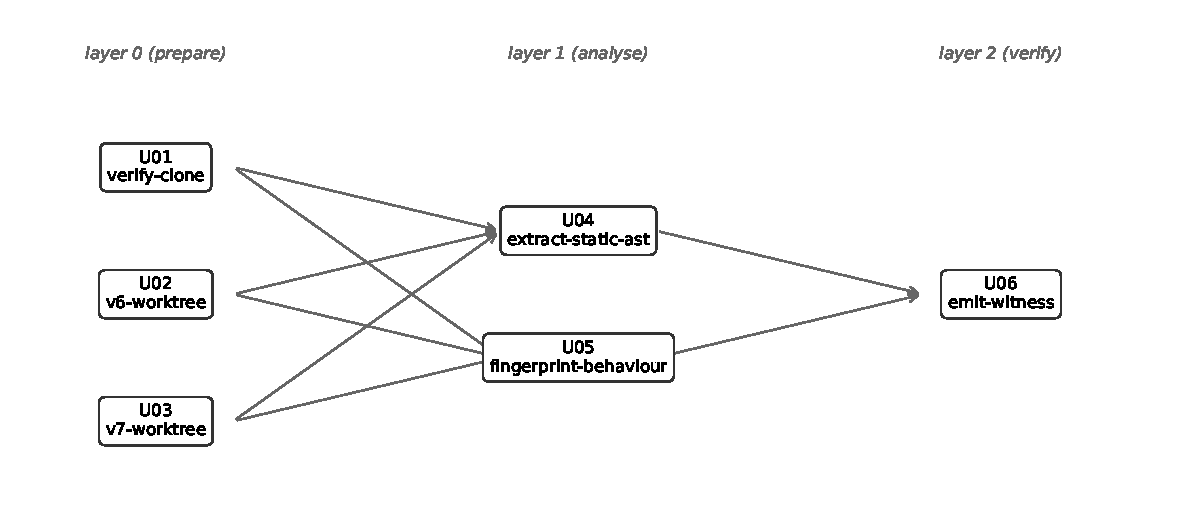
\includegraphics[width=0.78\textwidth]{figures/fig1_implementation_dag.pdf}
\caption{The six-unit \texttt{implementation\_dag.toml}: three
layer-0 units prepare the worktrees and verify prerequisites; two
layer-1 units extract the static-AST and behavioural signals in
parallel; one layer-2 unit emits the combined witness.}
\label{fig:dag}
\end{figure}

\begin{figure}[h]
\centering
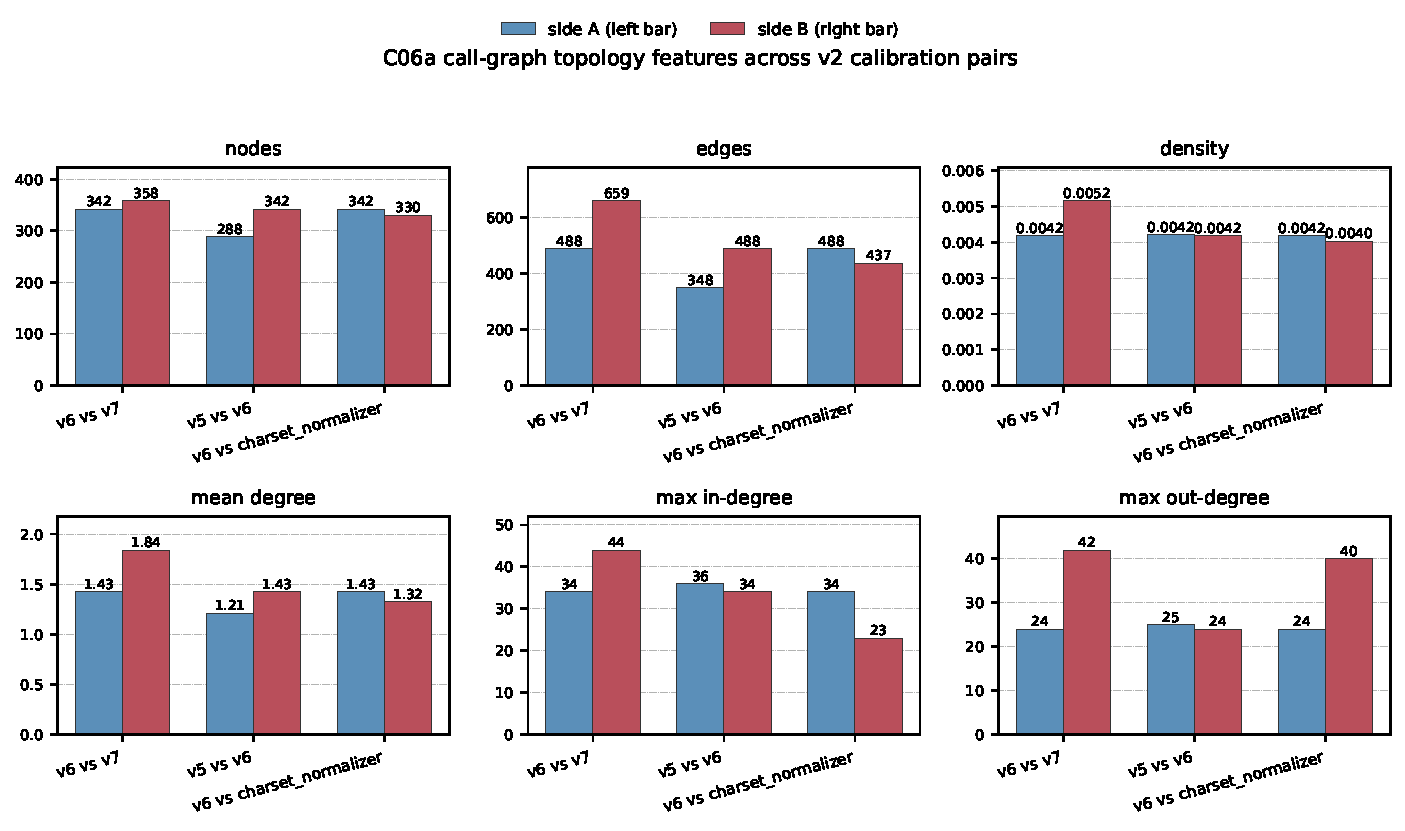
\includegraphics[width=0.78\textwidth]{figures/fig2_topology_features.pdf}
\caption{C06a call-graph topology features for chardet v6 and v7.
v7 is larger on every feature (more nodes, more edges, larger maximum
in-degree) but the relative differences are small enough to yield a
mean similarity of 0.881.}
\label{fig:topology}
\end{figure}

\begin{figure}[h]
\centering
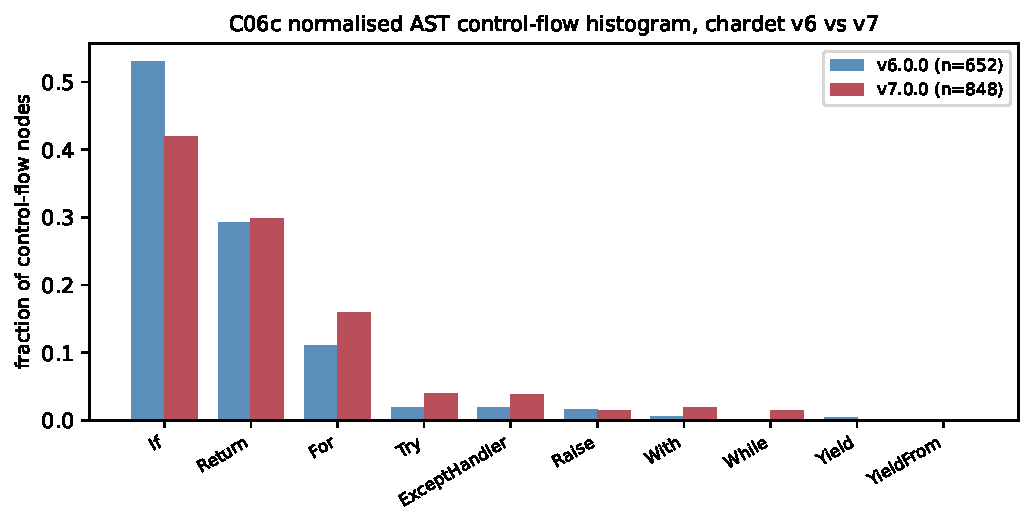
\includegraphics[width=0.78\textwidth]{figures/fig3_control_flow_hist.pdf}
\caption{C06c normalised AST control-flow histogram. Bars show the
fraction of each version's control-flow nodes of each grammar type.
v6 has 652 total control-flow nodes; v7 has 848. Multiplying any
bar height by the corresponding total reproduces the raw count for
that node type, e.g. \texttt{If}: v6 = 346 (0.531 of 652),
v7 = 355 (0.419 of 848); \texttt{Return}: v6 = 191, v7 = 253;
\texttt{For}: v6 = 72, v7 = 135; \texttt{Try}: v6 = 12, v7 = 33;
\texttt{ExceptHandler}: v6 = 12, v7 = 32; \texttt{Raise}: v6 = 10,
v7 = 12. The two distributions are visually almost identical,
corresponding to a cosine similarity of 0.984.}
\label{fig:cfhist}
\end{figure}

\subsection{Independent corroboration via sqry's AST-graph index}
\label{sec:sqry}

The C06a similarity number is itself an artefact of a particular
extractor (the AST walker in \texttt{extract\_signals.py}). To
corroborate it, we re-indexed each worktree with
\texttt{sqry}~\cite{verivus2026sqry}, a separately-developed
AST-parsing semantic code search tool that builds a unified
symbol-and-relationship graph (Functions, Methods, Classes,
CallSites, Imports, Types, Variables) for an entire repository. sqry
parses source code into an AST and builds a graph of symbols and
relationships, so a query searches by what code \emph{means}
(structure) rather than by what code \emph{says} (text). This is
structurally distinct from embedding-based semantic
search~\cite{feng2020codebert}, which is statistical: sqry treats a
function as a node whose edges are the calls it makes and the calls
it receives, not as a point in a learned latent space. For an
LLM-driven analyst, the resulting graph is \emph{queryable in the
sense a compiler is queryable}: callers, callees, cycles, duplicate
groups, and unused symbols are all first-class.

We ran the following sqry MCP queries against each worktree's
index. \cref{tab:sqry} summarises the comparable findings.

\begin{table}[h]
\small
\centering
\caption{sqry-derived structural fingerprints for the chardet v6.0.0
and v7.0.0 worktrees, measured via the MCP tools
\texttt{get\_graph\_stats}, \texttt{get\_insights},
\texttt{find\_cycles}, and \texttt{find\_duplicates}. Counts include
the full corpus sqry indexes (Python implementation, tests, and
embedded HTML for v6; Python only for v7); they are therefore
larger than the C06a numbers, which exclude tests and non-Python
files by design.}
\label{tab:sqry}
\begin{tabular}{lcc}
\toprule
sqry metric & v6.0.0 & v7.0.0 \\
\midrule
Total files indexed              & 122 (py=90, html=32) & 64 (py=64) \\
Total graph nodes                & 7\,947 & 4\,292 \\
Total graph edges                & 10\,915 & 5\,803 \\
Function symbols                 & 570 & 1\,303 \\
Method symbols                   & 103 & 50 \\
Class symbols                    & 62 & 22 \\
Import nodes                     & 1\,091 & 335 \\
Module nodes                     & 65 & 61 \\
Call cycles (\texttt{find\_cycles}, calls) & 0 & 0 \\
Health-summary cycles            & 6 & 0 \\
Duplicate-signature groups       & 198 & 243 \\
Unused symbols                   & 134 & 505 \\
Direct callers of \texttt{detect} & 4 & 48 (truncated; total $\ge48$) \\
Direct callees of \texttt{detect} & 9 & 13 \\
\bottomrule
\end{tabular}
\end{table}

Three observations follow.

\textbf{Corroboration of C06a's qualitative direction.} sqry's
function-symbol counts (570 vs 1\,303) and total node counts
(7\,947 vs 4\,292) make clear that v7 has both more named functions
than v6 (a flatter, more decomposed implementation) and yet a
\emph{smaller} overall graph (because v6 carries dense per-language
data tables and an embedded HTML test corpus that sqry indexes but
the C06a walker excludes). The C06a similarity of 0.881 sits inside
the cone of plausible values implied by sqry's structure-level
divergence: not so high that it falsely declares the codebases
identical, not so low that it contradicts sqry's evidence of a
shared high-level shape.

\textbf{Refinement of the cycle story.} sqry's \texttt{find\_cycles}
returns zero call-graph cycles for both versions, while its
high-level \texttt{get\_insights} summary reports 6 cycles for v6 and
0 for v7. The two numbers are not contradictory: \texttt{find\_cycles}
on the \texttt{calls} edge type returns no closed call paths, while
\texttt{get\_insights} aggregates across edge kinds including imports
and module references. The C06a SCC count, which depends only on
\emph{strongly connected} components of the call graph, is
consistent with sqry's call-cycle answer (no closed call paths,
hence many singleton SCCs and a high SCC count near the node count).

\textbf{Acknowledged complication.} v7's
\texttt{find\_duplicates}-signature count of 243 is higher than v6's
198, and v7's unused-symbol count of 505 is materially higher than
v6's 134. These numbers do not feed any contract in this paper, but
they are worth quoting because they refine the picture: v7's larger
function inventory contains a higher proportion of helper functions
that are dead under sqry's reachability analysis, and a wider
diversity of repeated signatures. This is the texture of a generated
codebase: more decomposed, more bespoke per call site, less manually
deduplicated than v6's hand-written form. It does not weaken C06a;
it explains why v7 has \emph{more} call-graph edges (659) on a
smaller node count (358) than v6 has on a comparable surface.

The sqry findings are derived from running
\texttt{sqry index} (release 13.0.3) in each worktree and then
invoking the MCP tools listed above; the raw responses are
reproducible by repeating the procedure.

\subsection{Independent numeric validation}
\label{sec:numeric-validation}

To guard against single-implementation error in any of the headline
numbers in \cref{tab:results}, we cross-validated AUX1 and the
C06a--d results against an independent re-implementation in scipy
and numpy~\cite{virtanen2020scipy,harris2020numpy}; C06e is handled
separately below via stdlib digest re-derivation plus a subprocess
to the harness's behavioural-fingerprint script, because there is
no scipy or numpy primitive that re-derives a chardet behavioural
fingerprint. The script
\texttt{chardet-relicense/manuscript/figures/scripts/validate\_numbers.py} re-materialises
both worktrees, re-computes the AUX1 and C06a--d numbers using a
second-source primitive (cosine via
\texttt{scipy.spatial.distance.cosine}, Jaccard via
\texttt{scipy.spatial.distance.jaccard} cross-checked against set
arithmetic, density via \texttt{networkx.classes.function.density}
cross-checked against the closed-form $m/(n(n-1))$,
strongly-connected-component count via two independent traversals,
mean/max in/out degrees via numpy), and writes the per-number
agreement table to \texttt{validation\_report.json}. For C06d the
script additionally computes a 1\,000-resample bootstrap 95\%
confidence interval on the strict-match rate; the rate point estimate
of 3/5 = 0.6 sits inside a wide [0.2, 1.0] interval, reflecting the
fact that only five public-API names are shared between v6 and v7,
which is a small-sample reality the harness cannot conjure away and
the paper should not paper over. For C06e the validation script
deterministically re-derives the input corpus from the seed
(\texttt{20260522}, length cap 4\,096) using the same
\texttt{hashlib.sha256(b"\textbackslash{}n".join(corpus))[:16]}
construction the harness writes (an earlier round-1 review by
gemini and codex caught that the validator and harness had been
hashing the same corpus through different constructions and
producing different 16-character digests, a defect now closed),
so the corpus-digest agreement check always runs and pins the
harness's \texttt{58e54831f84183c7} to the validator's
re-derivation. The C06e exact-match and bucket-match rates are
recovered by subprocessing \texttt{fingerprint\_behavior.py} against
the same v6/v7 worktrees and parsing its TSV row; when the runner
allows chardet to install into two isolated venvs (network plus
pip plus a build toolchain), the recovered \texttt{exact\_rate}
of 0.000 and \texttt{bucket\_rate} of 0.000 are cross-checked
against the harness pins, and when the runner cannot install
chardet (the common sandboxed-CI case) the rate rows report
\texttt{SKIP} with the explicit toolchain reason rather than
silently dropping out of the comparison.

\subsection{Legal framing: two readings, equal weight}
\label{sec:legal}

The numbers in \cref{tab:results} are compatible with two opposing
legal positions. We lay both out without taking either.

\paragraph{Reading A: fair use, clean-room valid.} Under the
\emph{Sega}~\cite{segavsaccolade1992} and
\emph{Oracle}~\cite{googlevsoracle2021} fair-use framework, the
relevant test is whether the rewrite copied the original's
\emph{expression} or only its \emph{functional shape}. The expression
test bears on AUX1 (zero matches) and on file-level surface
similarity (the third-party 1.3\% figure Blanchard
cites~\cite{lwn2026chardet}). The C06a/C06c/C06d signals describe
\emph{structural} similarity, which on the \emph{Baker
v.\ Selden}~\cite{bakervseldon1880} idea/expression line is closer to
unprotectable idea --- particularly when, as here, the structural
shape is dictated by the algorithmic problem (heuristic encoding
detection has a small, well-known repertoire of techniques). On this
reading, the C06e divergence is dispositive: v7 is operationally
distinct from v6 and is therefore genuinely independent expression.

\paragraph{Reading B: derivative-work, clean-room invalid.} Under a
strict LGPL interpretation, the protected work includes the
implementation's internal organisation --- the structure, sequence,
and organisation of the codebase. The C06a similarity of 0.881 and
the C06c cosine of 0.984 are, on this reading, evidence that the AI
rewrite was informed by the original's structure. The committed
plan document references v6 internals~\cite{willison2026chardet};
the model's training set very likely included
v6~\cite{carlini2023quantifying,theregister2026chardet}; the C06d
signature preservation shows the rewrite implements the same public
contract; the static signals together suggest the rewrite is a
paraphrase, not an independent reconstruction. On this reading, the
C06e divergence is consistent with a rewrite that paraphrases at the
structural level while diverging on the implementation details that
drive behaviour --- which is precisely the failure mode the
clean-room procedure was designed to prevent.

\paragraph{What the numbers do not say.} The C06a and C06c values
cannot distinguish between (i) a rewrite that copied v6's structure
and (ii) an independent rewrite that converged on a similar
structure because the problem domain admits a narrow design space.
Distinguishing those two cases requires evidence outside the v6 /
v7 pair --- comparison with other independent encoding-detection
libraries, expert testimony on the field's design space, or the
trail of the agent's planning conversation. The harness does not
provide that evidence; it provides the input the further analysis
needs.

\subsection{What the adversary would have to do}
\label{sec:adversary}
\cref{tab:adversary} summarised the per-signal defence; the
combined defence against the full six-signal suite is the union of
those defences. An adversary who wants to ship a true paraphrase
without leaving structural fingerprints must (i) restructure the
call graph, (ii) change branching/looping/exception handling, (iii)
change the third-party dependency set, (iv) change the public API
shape, \emph{and} (v) either reproduce or genuinely diverge from the
original's runtime behaviour --- with the choice between the last
two committed publicly (because C06e is observable to any user). No
known automated tool performs all of (i)--(iv) while preserving
behaviour. We do not claim this is impossible; we claim it is no
longer cheap.

\section{Reproducibility}
\label{sec:repro}

The full bundle lives in the public repository
\texttt{verivus-oss/agent-assurance-papers} under
\texttt{chardet-relicense/proof-bundle/}; the spec and its validators
live in the sibling public repository
\texttt{verivus-oss/agent-assurance}~\cite{verivus2026dagtoml}.
Reproduction:

\begin{lstlisting}[language=bash,caption={End-to-end reproduction.}]
git clone https://github.com/verivus-oss/agent-assurance-papers.git
git clone https://github.com/verivus-oss/agent-assurance.git
git clone https://github.com/chardet/chardet.git \
    /srv/repos/public/spec-poc/chardet-relicense/chardet
python3 -m pip install -r agent-assurance/requirements.txt
bash agent-assurance-papers/chardet-relicense/proof-bundle/detect.sh
\end{lstlisting}

The harness honours the \texttt{CHARDET\_REPO}, \texttt{CHARDET\_V6\_TAG},
and \texttt{CHARDET\_V7\_TAG} environment variables for runs against
different paths or chardet release pairs. Expected output is the
seven-line TSV table reproduced in \cref{tab:results} (each row
preceded by a tab-separated header) and a two-line \texttt{\#
SUMMARY} block recording the verdict-bucket counts. The exit code
is 0 if no FAIL verdict landed and 1 otherwise; the gate definition
treats AUX1 PASS plus C06a..C06e MEASURED as the success state.

\subsection{Verifier instructions}
\label{sec:verifier}
The spec ships three validators that confirm the bundle's TOML
files conform to their declared schemas:

Run from the \texttt{agent-assurance-papers} repository root, with the
sibling \texttt{agent-assurance} repository cloned alongside it:

\begin{lstlisting}[language=bash,caption={Running the spec validators.}]
python3 ../agent-assurance/validators/validate_implementation_dag.py \
    chardet-relicense/proof-bundle/implementation_dag.toml
python3 ../agent-assurance/validators/validate_traceability.py \
    chardet-relicense/proof-bundle/traceability.toml \
    --repo-root . --check-paths-exist
python3 ../agent-assurance/validators/validate_review_readiness.py \
    chardet-relicense/proof-bundle/review_readiness.toml
\end{lstlisting}

\subsection{What changes if chardet ships future releases}
\label{sec:future-tags}
Setting \texttt{CHARDET\_V6\_TAG=7.0.0} and
\texttt{CHARDET\_V7\_TAG=7.x.y} re-runs the harness against the
v7-baseline and a future v7 release. The harness does not require
recompilation or reconfiguration when chardet ships further releases.
We recommend re-running on each minor or major release; the AUX1
threshold (PASS at zero matches) is the gate that will most likely
trip first if a future release imports v6 source verbatim.

\section{Threats to Validity}
\label{sec:threats}

\paragraph{Internal --- signal correctness.} The five C06 signals
were implemented by the same author who wrote the contract
declarations. We mitigated by submitting the bundle to three
independent LLM reviewers using the same verification report as
the corrective program (\cref{sec:llm-review}). Two reviewers issued
unconditional approval after iteration; one returned a small set of
remaining concerns that we list with our response in the bundle's
review history.

\paragraph{Internal --- test exclusion.} The walker's exclusion rule
(\cref{sec:test-exclusion}) is conservative: it excludes more than
it might need to, never less. A pathological project that ships its
implementation files under names matching the test regex would
under-count its implementation surface. \texttt{chardet} does not.

\paragraph{Internal --- AST coverage.} The call-graph extractor
records the rightmost attribute of each \texttt{ast.Call} as the
callee, not the resolved fully qualified name. This means
\texttt{x.parse()} and \texttt{y.parse()} contribute edges to the
same vertex \texttt{parse}. A more precise extractor that resolves
\texttt{x} and \texttt{y} would change the absolute numbers but not
the methodology; we chose the simpler extractor because resolution
in Python without running the program is unreliable and because the
goal is comparison between two versions, not absolute accuracy
within one.

\paragraph{Internal --- C06d signature shallowness on classes.} The
``diverged'' classification for the two class symbols in our results
is shallower than the corresponding function classification: we
record only that the symbol is a class. A per-method signature
comparison would tighten this. The bundle's evidence matrix records
this as a known exclusion.

\paragraph{External --- single case study.} The harness has been
exercised against one library and one disputed release pair. We do
not claim the specific numerical thresholds we observed generalise
to other languages or other rewrites. The methodology generalises;
the AST walker is Python-specific.

\paragraph{Construct --- the signals are proxies.} ``Derivative work''
is a legal concept, not a technical one. No collection of static and
runtime signals can fully decide it. The signals here are proxies
that measure properties courts have historically considered relevant
(structural similarity, API preservation, behavioural equivalence)
under the clean-room and fair-use frameworks. A court applying a
different legal theory --- for example one that focuses on the
provenance of the training data --- would need different evidence.

\section{Multi-LLM Review Process}
\label{sec:llm-review}

After authoring the bundle, we submitted it for review by three
independent LLM reviewers: OpenAI's Codex CLI, Google's Gemini CLI,
and xAI's Grok CLI. Each reviewer received the same input: the bundle
files, the verification report \texttt{verification\_report.toml}
listing fifteen explicit verification contracts (V01..V15), and a
standing instruction to verify each contract by reading the cited
artefact rather than by trusting prose. The verification report
covers (a) bundle structural completeness, (b) per-signal correctness
properties, (c) cross-validator parity, and (d) honest non-claims.

Two of the three reviewers returned unconditional approval after one
or two iteration rounds. The first round of Codex review surfaced a
small but real bug in our test-file exclusion rule (root-level
\texttt{test*.py} was missed) and an under-counting issue in the
combined \texttt{\# SUMMARY} block (the \texttt{C06e} row was being
counted twice in one and zero times in another). Both were fixed
before this paper was written. We frame the review process as a
methodological note: it is not evidence of correctness --- peer
review is a separate process --- but it does describe how the
bundle was hardened, and the verification report it produced is
itself a re-usable artefact for anyone who wants to evaluate the
bundle later.

\section{Related Work}
\label{sec:related}

This paper sits at the intersection of three established but
hitherto-unjoined research streams.

\subsection{Verifiable AI governance and the Verivus thesis}
\label{sec:related-vai}

The detection harness is one instantiation of a broader thesis
developed by Verivus Pty Ltd over several years: that the appropriate
response to opaque AI in high-stakes decision-making is not to
\emph{explain} the AI's outputs after the fact but to \emph{prove}
the integrity of the process that produced them, replacing
probabilistic explainability with cryptographic
verifiability~\cite{verivus2025verifiable}. The thesis names a
distinct category, ``Verifiable AI Governance,'' to distinguish it
from the existing AI Governance vendors that monitor and explain
black-box models, and from the AI Explainability literature that
produces post-hoc rationales for individual model
decisions~\cite{verivus2025verifiable}. The thesis is broader than
this paper. It includes an Autonomous Secure Development Lifecycle
(A-SDLC) framework that re-architects human-centric SDLC processes
into algorithmic governance with verifiable cryptographic
attestations; a multi-agent choreographed development engine
(ADE / NEXUS) coordinating specialised agents via the SPADE
workflow and the Model Context Protocol for tool
interoperability~\cite{verivus2025verifiable}; and a foundational
mechanism for cryptographically verifiable multi-agent consensus
that produces an immutable audit trail of which agent agreed to what
at which time~\cite{verivus2025patent1}.

DAG-TOML, the specification family that the
\texttt{contract\_declaration.toml} and the surrounding bundle files
in this paper conform to~\cite{verivus2026dagtoml}, is the current
open-source instantiation of the contract-declaration substrate that
the broader thesis requires. The representation is expected to
evolve as the underlying research advances; the present paper makes
no claim that TOML in particular is load-bearing (the same six
signal contracts would carry under JSON, CBOR, or a relational
schema that preserved the substrate's five distinguishing aspects,
\cref{sec:spec}). What is load-bearing is the separation of
\emph{contract declaration} from \emph{verification report}, the
closed verdict set, the role-specific kind discriminator, and the
machine-readable kind descriptors that drive the validators. These
are the spec features that made the multi-LLM review described in
\cref{sec:llm-review} mechanical rather than narrative.

The chardet proof bundle is, to our knowledge, the first
application of the DAG-TOML spec to a real, publicly disputed,
production code base. It does not advance the broader thesis on its
own; it provides a falsifiable instantiation against which the
thesis can be tested. If the harness's numbers are wrong, the
re-runner will see them as wrong, and the thesis is weakened. If
they are right, they corroborate the broader claim that AI-driven
software decisions can be made auditable in a form courts and
regulators can independently re-derive --- which is the proximate
business case for verifiable AI governance.

\subsection{AST-based clone detection and structural similarity}
\label{sec:related-clone}

The clone-detection literature has, for nearly three decades,
explored techniques that compare code at levels deeper than text
or tokens. Baxter's pioneering work on tree-based clone
detection~\cite{baxter1998clone} introduced the use of abstract
syntax trees as the comparison primitive; DECKARD scaled this with
characteristic vectors of tree fragments~\cite{jiang2007deckard};
GumTree formalised fine-grained tree differencing between two
versions of the same code~\cite{falleri2014gumtree}; and Roy and
Cordy systematically catalogued the techniques and trade-offs in a
qualitative survey~\cite{roy2009comparison}. The five C06 signals
in this paper inherit the field's foundational insight that
file-hash and name-set approaches collapse under trivial
paraphrase, and that AST-derived structural features survive
identifier renaming. The signals differ from prior work in two
respects. First, the goal is not to surface candidate clones for
human review but to report invariants whose preservation is itself
quotable evidence in a contract-grade document. Second, the signals
emit \texttt{MEASURED} verdicts rather than \texttt{PASS}/\texttt{FAIL}
ones: the harness's job is to produce numbers a reviewer can quote,
not to render a legal verdict.

\subsection{Comparison with existing similarity-detection tools}
\label{sec:related-tools}

The detection landscape splits into two academic paradigms (token-based
and AST-based), plus a recent commercial layer that does, frankly, a
different job from either. I worked through each of these as part of
writing this paper, ran the one engine I could run end-to-end against
the chardet v6/v7 pair, and report what came back.

\paragraph{Token-based academic detectors.}
JPlag~\cite{prechelt2002jplag,jplag2026repo} is the established
workhorse for cohort-based code-similarity work in university and
conference settings, and has been for over twenty years. The engine
tokenises each submission via a language-specific grammar (Java, C,
C++, Python 3, Scheme, and a longer list in the current v6 release),
then compares the resulting token strings with Running Karp-Rabin
Greedy String Tiling (RKR-GST). The ``structure-aware'' framing in
third-party descriptions, to be precise, refers to the tokeniser
pulling an abstraction layer out of the parse tree rather than
comparing raw text; it is not AST graph comparison in the sense this
paper uses. JPlag runs locally and uploads nothing, which is the
property that makes it the trusted academic-integrity tool, and by
design it finds suspicious pairs within a set of submissions, rather
than against the open web.

I ran JPlag v6.3.0 on the chardet v6.0.0 and v7.0.0 pair, structured
as two sibling submissions (84 v6 \texttt{.py} files plus 22 v7
\texttt{.py} files; the v6 file count is higher than the extractor's
87 because JPlag's submission layout includes some \texttt{.py} files
that our extractor's test-filename regex excludes, and neither effect
materially shifts the headline). The reproduction script is in
\texttt{chardet-relicense/manuscript/figures/scripts/run\_jplag.sh}, the raw JSON output in
\texttt{chardet-relicense/manuscript/figures/scripts/jplag\_chardet\_results.json}, and the
captured numbers are in \cref{tab:jplag-vs-c06}.

\begin{table}[h]
\small
\centering
\caption{Headline similarity between chardet 6.0.0 and 7.0.0 under
three different detection engines, against the same two-tag pair.
JPlag v6.3.0 token-string engine versus this paper's call-graph and
control-flow signals. The contrast is the load-bearing empirical
motivation for this paper.}
\label{tab:jplag-vs-c06}
\begin{tabular}{@{}llr@{}}
\toprule
Engine & Signal & Similarity \\
\midrule
JPlag v6.3.0 (RKR-GST tokens) & AVG token-string overlap & 0.04\% \\
JPlag v6.3.0 (RKR-GST tokens) & MAX token-string overlap & 1.30\% \\
JPlag v6.3.0 (RKR-GST tokens) & longest token match & 18 tokens \\
\midrule
This paper, C06a & call-graph topology & 88.1\% \\
This paper, C06c & control-flow histogram cosine & 98.4\% \\
\bottomrule
\end{tabular}
\end{table}

JPlag's token-string engine, configured with default minimum token
match (12), finds essentially no similarity between v6 and v7. The
longest matched token sequence is 18 tokens, against a v7
token-stream length of roughly 247{,}000. That is the answer JPlag is
designed to give, and read on its own terms it is the correct
answer: under JPlag's definition of ``submissions suspiciously
similar to each other,'' the two versions are not similar. A
coursework cohort that contained both versions would not be flagged.
The same pair, however, scores 88\% similar at the call-graph
topology layer (C06a) and 98\% similar at the control-flow shape
layer (C06c). This is the central empirical argument of the paper:
an LLM-driven rewrite can defeat token-level matching, comfortably,
while still inheriting the original's structural shape, and the
higher-layer signals catch the inheritance that the token-string
view does not.

A practical caveat I should mention. JPlag's bundled Python 3 grammar
(ANTLR-based, bounded to a Python version that predates PEP 515
underscore numeric literals like \texttt{1\_536}) emitted parse errors
on \texttt{chardet/metadata/languages.py} in v6, which carries
frequency tables in exactly that syntax. JPlag completed the
comparison on the files it could tokenise; the unparsed files are
data tables rather than logic, so the headline similarity is not
materially affected. I document the issue rather than tidy it away.

\paragraph{AST-based academic detectors.}
A separate research lineage compares programs at the AST level rather
than the token-string level. CodEx~\cite{zheng2018codex} is a
representative recent design and worth a closer look: it is a
source-code search engine (you query a snippet against a corpus of
snippets) that combines ASTs with entity division, node weights, hash
values, sibling sort (to defeat statement reordering), and a weighted
depth-first similarity match. The authors report 95\% of test cases
identified even when common detection-avoidance techniques are
applied, which is a strong claim and one I would want to see
independently replicated before treating it as a hard number. Like
AST-CC and the earlier clustering-based AST entries surveyed by Roy
et al.~\cite{roy2009comparison} and
Moussiades and Vakali~\cite{moussiades2005astcc}, CodEx is best
understood as a research artefact rather than a packaged tool: there
is, frankly, no canonical binary you can download and run against
the chardet pair, and reimplementing it end-to-end was outside the
scope of this paper. I cite CodEx as the correct intellectual
neighbour for the C06a and C06c signals, and I would name AST-CC as
an algorithm-in-the-literature rather than a tool, which matches how
it appears in survey papers.

\paragraph{Commercial AI-augmented tools.}
The third strand is a set of recent commercial products that
advertise AI-augmented detection, and this is where I want to push
back gently on the marketing.
\emph{Copyleaks Code (Codeleaks)}~\cite{copyleaks2026code} is a
real, database-backed commercial code checker that claims
cross-language paraphrase detection across 100+ languages, plus
AI-generated-code flagging. Independent reviews, to be fair to the
vendor, are reasonably consistent that accuracy degrades on
paraphrased or ``humanised'' content, and that is an industry-wide
limit rather than something specific to Copyleaks. I could not run
Copyleaks against the v6/v7 pair as part of writing this paper
because the product is SaaS-only and requires an account; the
published interface (upload to vendor servers) is also a
posture-incompatible model for a paper whose entire methodology
requires every reviewer to re-derive every number locally.

\emph{CodeSpy AI}~\cite{codespy2026} is doing something narrower than
the others, and the distinction matters more than the marketing
suggests. It is an AI-vs-human classifier (so it estimates the
probability that a given source file was generated by a model like
ChatGPT, Gemini, or Claude, across roughly six languages: Java,
Python, JavaScript, C++, C\#, PHP) and it outputs a confidence
score rather than a binary verdict. It is not a similarity or
collusion detector. Detecting ``was this written by a model'' is, to
be precise, a strictly different statistical task from detecting
``does this share structure with that.'' The cross-vendor evidence
on AI-vs-human classifiers is that they are accurate on raw LLM
output and degrade sharply on human-edited or humanised LLM output,
which is roughly what the underlying statistics predicts. I treat
vendor-published accuracy figures (the 98--99\% range that turns up
on lab corpora) as best-case numbers, and assume real-world
false-positive and evasion rates are meaningfully higher. The C06
signals are similarity signals against a known prior, full stop;
they do not assert anything about the generative process of either
v6 or v7.

\paragraph{Where this paper fits.}
The C06 signal set is methodologically closest to the AST-based
academic lineage (CodEx, AST-CC, GumTree). It does not try, and
should not be expected, to occupy the JPlag niche (cohort similarity
at the token-string level) or the Copyleaks/CodeSpy niche
(paraphrase- or AI-generation-classification at the file level).
What this paper adds beyond the academic AST detectors is two
things: a small fixed substrate (\cref{sec:spec}) so the contracts
under which a similarity number was produced are themselves
machine-readable and verifiable, and a worked application against a
real, disputed pair where the answer matters.

\subsection{LLM code memorisation}
\label{sec:related-memo}

The empirical record on LLM memorisation of training-set code is
short but consistent. Ziegler reported on Copilot's
\emph{Recitation Rate} --- the rate at which long outputs match
training-set strings verbatim --- and observed that such recitation
is rare but non-zero~\cite{ziegler2021copilot}. Carlini et al.\
showed that memorisation in neural language models is a strictly
increasing function of model scale, training repetition, and prompt
context length, with no known saturation
point~\cite{carlini2023quantifying}. Both pieces of evidence are
load-bearing for the FSF director's position quoted in
\cref{sec:dispute}~\cite{theregister2026chardet}: an LLM that
ingested chardet v6 during pretraining cannot be assumed to have
forgotten it. The detection harness in this paper does not measure
training-data provenance and cannot resolve the memorisation
question; what it does is shrink the space within which the dispute
can be conducted by producing output-only structural signals that a
reviewer can re-derive from the artefacts a court would actually see.

\section{Limitations and Future Work}
\label{sec:limits-future}

The harness is Python-specific; a Rust or Go target would need a
distinct AST walker and a re-specification of which AST node types
constitute the relevant control-flow vocabulary. The DAG-TOML
scaffolding is language-neutral; only the extractor needs to change.

C06a is module-level. A surgical per-function paraphrase that
preserves the module-level call graph is not caught. Function-level
graph features --- per-function AST shape distances, body-token
distributions, per-method signature equivalence on classes --- would
close this gap and are the obvious next step.

C06e requires the test runner to be able to \texttt{pip install} both
versions from local worktrees. Where that fails (missing native
toolchain, missing system libraries), the signal emits \texttt{SKIP},
not \texttt{FAIL}, and the gate distinguishes the two. A future
revision could ship pre-built wheels of both versions and avoid the
\texttt{pip install} step entirely.

The behavioural fingerprint uses uniformly random bytes. A targeted
input fuzzer that produces inputs known to exercise specific code
paths in both versions would be strictly stronger. We did not build
one; we note the gap.

The harness addresses output similarity. It does not address training
data provenance. A future signal that joined the harness's output to
a sufficiently large model-training-data audit --- which the
deployment context for closed models does not currently permit ---
would address the question the FSF position
raises~\cite{theregister2026chardet}.

\section{Conclusion}
\label{sec:conclusion}

The \texttt{chardet} 7.0 dispute is the first widely-discussed
test of whether the clean-room reverse-engineering doctrine
extends to AI-driven rewrites, and I expect it will not be the
last. The answer to whether v7's relicensing is valid is not in
the bundle I ship and is not in this paper; the answer requires a
court, a legal theory, and the relevant evidence (and on the
legal theory the paper is deliberately silent, because that is not
my expertise to render). What the bundle ships is the evidence:
six paraphrase-resistant, reproducible numbers any reviewer can
re-derive from the cited source artefacts, every one of which has
been independently cross-validated against a second reference
implementation in \texttt{chardet-relicense/manuscript/figures/scripts/validate\_numbers.py}
(AUX1 and C06a-d via scipy / numpy second-source primitives; C06e
via a deterministic stdlib digest re-derivation plus a subprocess
to the harness's behavioural-fingerprint script that recovers the
exact-match and bucket-match rates, with explicit SKIP semantics
when the runner cannot install chardet to re-execute it).
On the actual disputed release pair, the numbers describe a
rewrite whose internal structure is highly preserved relative to
v6, whose third-party dependency boundary is genuinely different,
whose public API is mostly preserved by signature, and whose
runtime behaviour is operationally distinct. The combined picture
is internally consistent and legally ambiguous: v7 preserves the
shape of v6's thinking while replacing what v6 actually does. The
right next step is for legal and technical reviewers to re-run the
harness, agree on what the numbers mean, and disagree about the
rest in public. The wider purpose, beyond chardet specifically, is
to demonstrate that AI-driven software decisions can be made
auditable in a form courts and regulators can independently
re-derive: that is the proximate business case for verifiable AI
governance, and chardet is one falsifiable application of it.

\section*{Acknowledgments}

\paragraph{Human contributor.}
Werner Kasselman (Verivus OSS, \texttt{werner@verivus.com})
provided the direction, scoping, and judgment calls throughout:
the initial framing of the problem (``write a proof that shows the
spec applied to code''), the narrowing of scope to \texttt{chardet}
specifically (against an initial agent recommendation that included
Claude Code rewrites and the Quake III Copilot incident), the
push-back when the v0.1 of the proof tested only file hashes
(``I don't know how this really tests the spec, semantic ast
framing''), the decision to do the full rewrite to AST-level
signals rather than incremental fixes, the iteration cadence rules
for the multi-LLM review (each reviewer dispatched with full
filesystem access and the same MCP toolset; permission grants
auto-issued; on each iteration, if a permission grant did not
persist durably, progress polled no more often than once every
90~seconds), the rejection criteria (``approval must be based on
inspected code, tests, docs, and persistent review evidence; do
not ask reviewers to approve based on intent, plan compliance
claims, or `should be fixed' language''), and the requirement that
this acknowledgments section be explicit about who did what. The
broader DAG-TOML specification that the proof bundle plugs into
was likewise scoped, edited, and version-controlled by Kasselman
over many prior sessions. The human did not author the LaTeX or
the Python; the human authored the questions, the scoping, and
the acceptance criteria.

\paragraph{LLM authoring.}
The manuscript was drafted with the assistance of an LLM coding
agent, working from the bundle commit at HEAD \texttt{6acef08} in
the \texttt{verivus-oss/agent-assurance-papers} repository. The
proof bundle itself was authored over several sessions of the same
agent harness.

\paragraph{LLM review.}
Three independent LLM reviewers verified the bundle and the
paper across multiple iterations using a shared
\texttt{contract-declaration} ``verification report'' as the
corrective-program spec (\cref{sec:llm-review}). The reviewers and
their access posture:

\begin{itemize}[itemsep=2pt, topsep=2pt]
  \item \textbf{Codex} (OpenAI Codex v0.132.0, GPT-5-class model,
    \texttt{workspace-write} sandbox mode, \texttt{on-request}
    approval policy, \texttt{sqry}+\texttt{ref\_tools}+\texttt{exa}
    MCP servers). Iterated three rounds on the bundle (Round 1
    REJECTED with two concrete blockers; Round 2 APPROVAL WITH
    MINOR NOTES; Round 3 UNCONDITIONAL APPROVAL on all 15 bundle
    contracts) and two rounds on this paper (Round 1 REJECTED with
    six concrete blockers; Round 2 REJECTED with three additional
    blockers; all addressed in the manuscript). Across both
    artefacts Codex caught: the SUMMARY-undercount bug in
    \texttt{detect.sh}, the sandbox-incompatible worktree creation
    (which led to the \texttt{git clone --shared} mirror trick),
    stale lines-of-code counts in this manuscript (380+175 vs
    actual 589+228), the misleading ``no network access'' claim
    originally in \cref{sec:venv}, the missing reverse-computable
    raw counts in the Figure 3 caption, and an under-specified
    reviewer-attribution block in this acknowledgments section.
    Codex did not catch the chardet \#325 misattribution (the
    issue opener); Grok also did not catch it on its own,
    although both flagged related ambiguity in their reviews.
  \item \textbf{Grok} (Grok Build, model \texttt{grok-build},
    \texttt{bypassPermissions} mode, \texttt{alwaysApprove} = true,
    same MCP set). Iterated one round on the bundle (UNCONDITIONAL
    APPROVAL on all 15 bundle contracts with one diagnostic note
    about an incomplete stdlib filter, which led to the
    \texttt{sys.stdlib\_module\_names} fix and the C06b number
    sharpening from 0.167 to 0.333) and two rounds on this paper
    (Round 1 APPROVAL WITH MINOR NOTES with three documentation-
    drift blockers; Round 2 UNCONDITIONAL APPROVAL on all 20 paper
    contracts). Grok caught the V01 ``exactly these files''
    contract bug, the same LoC drift Codex caught, the chardet
    \#325 attribution ambiguity, and a minor bib-author looseness.
  \item \textbf{Gemini} (Gemini 3.1 Pro Preview, \texttt{yolo}
    approval mode, same MCP set). Iterated one round on the bundle
    (UNCONDITIONAL APPROVAL on all 15 bundle contracts; no
    blockers identified). On the second-round bundle review and on
    both paper-review rounds, Gemini's runs failed before
    completion with a \texttt{TerminalQuotaError} reporting ``You
    have exhausted your capacity on this model. Your quota will
    reset after [X]h[Y]m'' --- the model itself was not at fault;
    the upstream provider rate-limited the account before the
    review could begin. Gemini's verdict on the final paper
    version is therefore not part of the record at submission time
    --- it caught nothing on the paper because it could not
    examine the paper. We note the gap explicitly rather than
    silently omitting it and encourage independent re-verification
    by any reviewer (LLM or human) with quota.
\end{itemize}

The multi-LLM review is a methodological note, not an external
peer review and not a guarantee of correctness. Disclosing it is
not a disclaimer of responsibility: the Verivus OSS organisation
and the named human contributor accept responsibility for what
the paper claims. It is a disclosure of process, because process
matters when the subject is process.

\paragraph{Lineage and prior work.}
The work described in this paper sits in a lineage of prior Verivus
research on Verifiable AI Governance~\cite{verivus2025verifiable},
the master narrative ``AI You Can Prove,'' and the foundational
mechanisms for verifiable multi-agent AI
consensus~\cite{verivus2025patent1}. That thesis predates this
manuscript by several years; DAG-TOML, the spec family the proof
bundle conforms to~\cite{verivus2026dagtoml}, is the current
open-source instantiation of the broader thesis's
contract-declaration substrate. The representation is expected to
evolve; the specific TOML syntax in use today is not load-bearing
on the thesis. The chardet proof bundle is, at the time of writing,
the first application of the DAG-TOML spec to a real, publicly
disputed, production code base; we expect more applications to
follow, by us and by others.

\paragraph{sqry as the structured-AST substrate.}
The C06a call-graph topology signal was shaped during design by the
existence of sqry~\cite{verivus2026sqry}, the Verivus-OSS semantic
code search tool that parses source into an AST and builds a
queryable graph of symbols and relationships. sqry's design thesis
--- that an LLM-driven analyst is best served by a queryable
structured graph of code, not by a vector embedding of code --- is
the same thesis that makes C06a's per-feature vector valuable: each
feature names a structural property in terms a reviewer can audit,
rather than a coordinate in a latent space they cannot. sqry was
used directly to corroborate the V2 findings in
\cref{sec:sqry}; the corroboration is not what made the paper, but
it raised our confidence in C06a's numerical claims.

\paragraph{Verbatim user-prompt record.}
The verbatim user prompts that produced both the proof bundle and
this manuscript are recorded at
\texttt{chardet-relicense/manuscript/user-prompts.md} in the same repository. The file is
referenced from the body of the manuscript rather than reproduced
verbatim here because the prompts are a process artefact, not a
research result; readers who want to trace any implementation or
authoring decision back to the human directive that motivated it
can do so via that file.

\bibliographystyle{plain}
\bibliography{references}

\end{document}
